\PassOptionsToPackage{unicode=true}{hyperref} % options for packages loaded elsewhere
\PassOptionsToPackage{hyphens}{url}
%
\documentclass[english,man,mask]{article}
\usepackage{lmodern}
\usepackage{amssymb,amsmath}
\usepackage{ifxetex,ifluatex}
\usepackage{fixltx2e} % provides \textsubscript
\ifnum 0\ifxetex 1\fi\ifluatex 1\fi=0 % if pdftex
  \usepackage[T1]{fontenc}
  \usepackage[utf8]{inputenc}
  \usepackage{textcomp} % provides euro and other symbols
\else % if luatex or xelatex
  \usepackage{unicode-math}
  \defaultfontfeatures{Ligatures=TeX,Scale=MatchLowercase}
\fi
% use upquote if available, for straight quotes in verbatim environments
\IfFileExists{upquote.sty}{\usepackage{upquote}}{}
% use microtype if available
\IfFileExists{microtype.sty}{%
\usepackage[]{microtype}
\UseMicrotypeSet[protrusion]{basicmath} % disable protrusion for tt fonts
}{}
\IfFileExists{parskip.sty}{%
\usepackage{parskip}
}{% else
\setlength{\parindent}{0pt}
\setlength{\parskip}{6pt plus 2pt minus 1pt}
}
\usepackage{hyperref}
\hypersetup{
            pdfborder={0 0 0},
            breaklinks=true}
\urlstyle{same}  % don't use monospace font for urls
\usepackage{color}
\usepackage{fancyvrb}
\newcommand{\VerbBar}{|}
\newcommand{\VERB}{\Verb[commandchars=\\\{\}]}
\DefineVerbatimEnvironment{Highlighting}{Verbatim}{commandchars=\\\{\}}
% Add ',fontsize=\small' for more characters per line
\usepackage{framed}
\definecolor{shadecolor}{RGB}{248,248,248}
\newenvironment{Shaded}{\begin{snugshade}}{\end{snugshade}}
\newcommand{\AlertTok}[1]{\textcolor[rgb]{0.94,0.16,0.16}{#1}}
\newcommand{\AnnotationTok}[1]{\textcolor[rgb]{0.56,0.35,0.01}{\textbf{\textit{#1}}}}
\newcommand{\AttributeTok}[1]{\textcolor[rgb]{0.77,0.63,0.00}{#1}}
\newcommand{\BaseNTok}[1]{\textcolor[rgb]{0.00,0.00,0.81}{#1}}
\newcommand{\BuiltInTok}[1]{#1}
\newcommand{\CharTok}[1]{\textcolor[rgb]{0.31,0.60,0.02}{#1}}
\newcommand{\CommentTok}[1]{\textcolor[rgb]{0.56,0.35,0.01}{\textit{#1}}}
\newcommand{\CommentVarTok}[1]{\textcolor[rgb]{0.56,0.35,0.01}{\textbf{\textit{#1}}}}
\newcommand{\ConstantTok}[1]{\textcolor[rgb]{0.00,0.00,0.00}{#1}}
\newcommand{\ControlFlowTok}[1]{\textcolor[rgb]{0.13,0.29,0.53}{\textbf{#1}}}
\newcommand{\DataTypeTok}[1]{\textcolor[rgb]{0.13,0.29,0.53}{#1}}
\newcommand{\DecValTok}[1]{\textcolor[rgb]{0.00,0.00,0.81}{#1}}
\newcommand{\DocumentationTok}[1]{\textcolor[rgb]{0.56,0.35,0.01}{\textbf{\textit{#1}}}}
\newcommand{\ErrorTok}[1]{\textcolor[rgb]{0.64,0.00,0.00}{\textbf{#1}}}
\newcommand{\ExtensionTok}[1]{#1}
\newcommand{\FloatTok}[1]{\textcolor[rgb]{0.00,0.00,0.81}{#1}}
\newcommand{\FunctionTok}[1]{\textcolor[rgb]{0.00,0.00,0.00}{#1}}
\newcommand{\ImportTok}[1]{#1}
\newcommand{\InformationTok}[1]{\textcolor[rgb]{0.56,0.35,0.01}{\textbf{\textit{#1}}}}
\newcommand{\KeywordTok}[1]{\textcolor[rgb]{0.13,0.29,0.53}{\textbf{#1}}}
\newcommand{\NormalTok}[1]{#1}
\newcommand{\OperatorTok}[1]{\textcolor[rgb]{0.81,0.36,0.00}{\textbf{#1}}}
\newcommand{\OtherTok}[1]{\textcolor[rgb]{0.56,0.35,0.01}{#1}}
\newcommand{\PreprocessorTok}[1]{\textcolor[rgb]{0.56,0.35,0.01}{\textit{#1}}}
\newcommand{\RegionMarkerTok}[1]{#1}
\newcommand{\SpecialCharTok}[1]{\textcolor[rgb]{0.00,0.00,0.00}{#1}}
\newcommand{\SpecialStringTok}[1]{\textcolor[rgb]{0.31,0.60,0.02}{#1}}
\newcommand{\StringTok}[1]{\textcolor[rgb]{0.31,0.60,0.02}{#1}}
\newcommand{\VariableTok}[1]{\textcolor[rgb]{0.00,0.00,0.00}{#1}}
\newcommand{\VerbatimStringTok}[1]{\textcolor[rgb]{0.31,0.60,0.02}{#1}}
\newcommand{\WarningTok}[1]{\textcolor[rgb]{0.56,0.35,0.01}{\textbf{\textit{#1}}}}
\usepackage{graphicx,grffile}
\makeatletter
\def\maxwidth{\ifdim\Gin@nat@width>\linewidth\linewidth\else\Gin@nat@width\fi}
\def\maxheight{\ifdim\Gin@nat@height>\textheight\textheight\else\Gin@nat@height\fi}
\makeatother
% Scale images if necessary, so that they will not overflow the page
% margins by default, and it is still possible to overwrite the defaults
% using explicit options in \includegraphics[width, height, ...]{}
\setkeys{Gin}{width=\maxwidth,height=\maxheight,keepaspectratio}
\setlength{\emergencystretch}{3em}  % prevent overfull lines
\providecommand{\tightlist}{%
  \setlength{\itemsep}{0pt}\setlength{\parskip}{0pt}}
\setcounter{secnumdepth}{0}

% set default figure placement to htbp
\makeatletter
\def\fps@figure{htbp}
\makeatother

% Manuscript styling
\usepackage{upgreek}
\captionsetup{font=singlespacing,justification=justified}

% Table formatting
\usepackage{longtable}
\usepackage{lscape}
% \usepackage[counterclockwise]{rotating}   % Landscape page setup for large tables
\usepackage{multirow}		% Table styling
\usepackage{tabularx}		% Control Column width
\usepackage[flushleft]{threeparttable}	% Allows for three part tables with a specified notes section
\usepackage{threeparttablex}            % Lets threeparttable work with longtable

% Create new environments so endfloat can handle them
% \newenvironment{ltable}
%   {\begin{landscape}\begin{center}\begin{threeparttable}}
%   {\end{threeparttable}\end{center}\end{landscape}}
\newenvironment{lltable}{\begin{landscape}\begin{center}\begin{ThreePartTable}}{\end{ThreePartTable}\end{center}\end{landscape}}

% Enables adjusting longtable caption width to table width
% Solution found at http://golatex.de/longtable-mit-caption-so-breit-wie-die-tabelle-t15767.html
\makeatletter
\newcommand\LastLTentrywidth{1em}
\newlength\longtablewidth
\setlength{\longtablewidth}{1in}
\newcommand{\getlongtablewidth}{\begingroup \ifcsname LT@\roman{LT@tables}\endcsname \global\longtablewidth=0pt \renewcommand{\LT@entry}[2]{\global\advance\longtablewidth by ##2\relax\gdef\LastLTentrywidth{##2}}\@nameuse{LT@\roman{LT@tables}} \fi \endgroup}

% \setlength{\parindent}{0.5in}
% \setlength{\parskip}{0pt plus 0pt minus 0pt}

% \usepackage{etoolbox}
\makeatletter
\patchcmd{\HyOrg@maketitle}
  {\section{\normalfont\normalsize\abstractname}}
  {\section*{\normalfont\normalsize\abstractname}}
  {}{\typeout{Failed to patch abstract.}}
\makeatother
\shorttitle{Religious Disbelief}
\author{Will M. Gervais\textsuperscript{1}, Maxine B. Najle\textsuperscript{2}, Sarah R. Schiavone\textsuperscript{3}, \& Nava Caluori\textsuperscript{4}}
\affiliation{
\vspace{0.5cm}
\textsuperscript{1} University of Kentucky\\\textsuperscript{2} BlueLabs Analytics\\\textsuperscript{3} University of California-Davis\\\textsuperscript{4} University of Virginia}
\authornote{

Correspondence concerning this article should be addressed to Will M. Gervais, UK Psychology, Lexington, KY. E-mail: will.gervais@gmail.com}
\keywords{atheism; religion; culture; evolution; dual inheritance theory\newline\indent Word count: 8031}
\DeclareDelayedFloatFlavor{ThreePartTable}{table}
\DeclareDelayedFloatFlavor{lltable}{table}
\DeclareDelayedFloatFlavor*{longtable}{table}
\makeatletter
\renewcommand{\efloat@iwrite}[1]{\immediate\expandafter\protected@write\csname efloat@post#1\endcsname{}}
\makeatother
\usepackage{csquotes}
\ifnum 0\ifxetex 1\fi\ifluatex 1\fi=0 % if pdftex
  \usepackage[shorthands=off,main=english]{babel}
\else
  % load polyglossia as late as possible as it *could* call bidi if RTL lang (e.g. Hebrew or Arabic)
  \usepackage{polyglossia}
  \setmainlanguage[]{english}
\fi

\date{}

\begin{document}

\hypertarget{background}{%
\section{Background}\label{background}}

Religion is a bit of an evolutionary puzzle. Organisms like ants and aardvarks tend not to engage in painful and costly collective rituals to prove their faith in unseen ant and aardvark pantheons, respectively. It is intriguing, then, that these behaviors are cross-culturally ubiquitous in humans. Evolutionary approaches to religion have proliferated in recent years ({\textbf{???}}; {\textbf{???}}; {\textbf{???}}; {\textbf{???}}; {\textbf{???}}), and different theories make starkly different predictions about the existence, nature, and origins of religious disbelief. Thus, the origins of disbelief are a crucial testing ground for different theories of religion. Here we test predictions from three prominent theoretical frameworks (outlined in Table 1): secularization, cognitive byproduct, and an emerging dual inheritance (gene-culture coevolutionary) model of religion ({\textbf{???}}) that views both cognitive adaptations and specific cultural learning mechanisms ({\textbf{???}}) as key to the transmission of either faith or atheism ({\textbf{???}}; {\textbf{???}}; {\textbf{???}}; {\textbf{???}}). This project situates the study of religious disbelief firmly within established theoretical frameworks for studying the evolution of human behavior and contributes to broader discussions of the role of transmitted versus evoked culture in core aspects of human nature ({\textbf{???}}).

Religion simultaneously unites and divides like few other aspects of social life. The sectarian conflicts between groups of religious believers may obscure a more fundamental schism: that between believers and atheists. Atheists---merely people who do not believe in the existence of a God or gods---constitute a large and perhaps growing proportion of earth's human population. A prominent estimate from about a decade ago ({\textbf{???}}) posits the existence of 500-700 million atheists globally. This estimate is in all likelihood a drastic underestimate ({\textbf{???}}). Atheism prevalence estimates rely on census and polling data that infer individual beliefs from their self-reports. However, there is potent anti-atheist stigma that transcends national and religious boundaries ({\textbf{???}}; {\textbf{???}}; {\textbf{???}}; {\textbf{???}}; {\textbf{???}}): even atheists harbor some intuitive moral distrust of atheists worldwide ({\textbf{???}}). Thus, while it is safe to assume that self-reported atheists do not believe in God, it is probably also safe to assume that a great many people privately disbelieve without openly admitting their atheism. Consistent with this, people routinely overreport their religious practices ({\textbf{???}}), and indirect measurement of atheism in the USA reveals a potentially large gulf between some indirect (\textasciitilde{}26\%) and direct (\textasciitilde{}3\%) estimates of atheist prevalence ({\textbf{???}}). Combining direct estimates and inferences drawn from the few available indirect estimates, we predict that upwards of 2 billion people on earth may in fact be atheists. Many evolutionary theories of religion posit a universal or near-universal implicit theism ({\textbf{???}}; {\textbf{???}}; {\textbf{???}}; {\textbf{???}}), and may thus be fundamentally incompatible with global atheism that is simultaneously prevalent and deliberately concealed. Therefore, sustained research into the psychological origins of disbelief is necessary to test key assumptions of various evolutionary and cultural theories of religion.

\hypertarget{four-pathways-to-atheism}{%
\subsection{Four Pathways to Atheism}\label{four-pathways-to-atheism}}

While it is clear that a large and perhaps unrecognized proportion of the global population does not believe in gods, what cognitive, motivational, and cultural factors yield religious disbelief? Distinct research trajectories have considered the preconditions for sustained belief in any given god. To currently believe in a god, one 1) must be able to mentally represent gods ({\textbf{???}}; {\textbf{???}}; {\textbf{???}}; {\textbf{???}}), 2) must be dispositionally or situationally motivated to believe in some gods ({\textbf{???}}; {\textbf{???}}), 3) must receive credible cultural cues that some gods are real ({\textbf{???}}; {\textbf{???}}; {\textbf{???}}; {\textbf{???}}), and 4) must maintain this intuitive ({\textbf{???}}; {\textbf{???}}; {\textbf{???}}) belief over time. Tweaks to any of these four components may instead yield disbelief in gods. Separate lines of research partially support this supposition. First, it takes fairly advanced mentalizing abilities---the core cognitive faculty that enables us to mentally represent other minds and their contents---to conceptualize gods, and \emph{mindblind atheism} describes the pattern whereby individual differences in advanced mentalizing abilities predict religious disbelief ({\textbf{???}}; {\textbf{???}}) in at least some samples ({\textbf{???}}). Second, \emph{apatheism} describes the pattern whereby, although people are highly religiously motivated when life is insecure, unstable, and unpredictable, existential security instead predicts reduced religiosity ({\textbf{???}}; {\textbf{???}}). Third, \emph{inCREDulous atheism} describes the pattern whereby a lack of credibility enhancing displays (CREDs) ({\textbf{???}}) that one ought to believe in any gods is a good global predictor of atheism ({\textbf{???}}; {\textbf{???}}; {\textbf{???}}). Finally, \emph{analytic atheism} describes the pattern whereby people who reflectively override their intuitions tend to be less religious than those who \enquote{go with their guts} ({\textbf{???}}; {\textbf{???}}; {\textbf{???}}), although the magnitude and consistency of this relation is debatable ({\textbf{???}}). Although these four potential pathways to atheism relate to religious disbelief in isolation, little work considers their operation in conjunction ({\textbf{???}}). Prominent theoretical perspectives place different emphasis on the role of mindblind atheism, apatheism, inCREDulous atheism, and analytic atheism, thus the relative predictive strength of each pathway can help adjudicate between the respective theories.

\hypertarget{prominent-theoretical-approaches}{%
\subsection{Prominent Theoretical Approaches}\label{prominent-theoretical-approaches}}

Prominent theoretical approaches make rather divergent predictions about which pathways to atheism (mindblind, apatheism, inCREDulous, or analytic) are most important. First, secularization models ({\textbf{???}}; {\textbf{???}}; {\textbf{???}}) posit that increases in existential security (wealth, health, education, etc.) reduce religious motivation; this approach is common in sociology of religion ({\textbf{???}}) and in social psychology under the banner of compensatory control ({\textbf{???}}; {\textbf{???}}). Second, cognitive science of religion and evolutionary psychology often view religion as a cognitive byproduct of other mental adaptations ({\textbf{???}}; {\textbf{???}}; {\textbf{???}}), such as mind perception ({\textbf{???}}) or predator detection.\footnote{Though highly cited and widely discussed, there is a lack of actual empirical evidence supporting a Hyperactive Agency Detection Device and its contribution to religious cognition. Anecdotally, many-to-most graduate students in cognitive science of religion have tried these studies to no avail.} In this view, challenges in the core cognitive faculties underlying such adaptations (e.g., advanced mentalizing) would predict disbelief, but the primary route to disbelief is people overriding their religious intuitions via effortful cognitive reflection.\footnote{Prominent scholars of this tradition claim, for example, that atheism \enquote{require{[}s{]}\ldots{}cognitive effort} ({\textbf{???}}) and that \enquote{disbelief is generally the result of deliberate, effortful work} ({\textbf{???}}), strong claims for the primacy of analytic atheism.} Finally, dual inheritance models incorporate insights from the byproduct account while also drawing heavily upon work in cultural evolution ({\textbf{???}}; {\textbf{???}}; {\textbf{???}}). Cultural evolutionary models highlight the social learning processes ({\textbf{???}};; {\textbf{???}}; {\textbf{???}}) underpinning religious beliefs ({\textbf{???}}; {\textbf{???}}; {\textbf{???}}; {\textbf{???}}; {\textbf{???}}) and disbelief, and largely predict that context-biased social learning---especially CREDs ({\textbf{???}})---would be strongly associated with degrees of religious belief ({\textbf{???}}). The dual inheritance approach recognizes that evolved cognitive biases can generate content biases that canalize religious cognition, but context-biased learning may instead predict degrees of belief and disbelief ({\textbf{???}}). Our dual inheritance approach predicts that CREDs would be most important, followed by other factors such as cognitive reflection, mentalizing, and perhaps existential security. Table 1 depicts predictions derived from each of these perspectives. By simultaneously considering mindblind atheism, apatheism, inCREDulous atheism, and analytic atheism, we are able to evaluate the suitability of four prominent theoretical approaches from separate academic subdisciplines for understanding the origins of religious disbelief.

\begin{table}[!h]

\caption{(\#tab:predictions table)Predictions From Prominent Theories}
\centering
\begin{tabular}[t]{>{\bfseries}llrrrr}
\toprule
Theory & Discipline & mindblind & apatheist & inCREDulous & analytic\\
\midrule
Secularization & Sociology \& Social Psych &  & + + + + &  & \\
Cognitive Byproduct & Ev Psych \& Cog Sci Rel & + + & + &  & + + +\\
Dual Inheritance & Gene-Culture Coevolution & + & indirect & + + + + & + +\\
\bottomrule
\multicolumn{6}{l}{\textit{Note: }}\\
\multicolumn{6}{l}{+ symbols indicate the predicted strength of each pathway to atheism, by theory}\\
\multicolumn{6}{l}{\textsuperscript{1} mindblind = relatively lower in advanced mentalizing}\\
\multicolumn{6}{l}{\textsuperscript{2} apatheist = relatively more existentially secure}\\
\multicolumn{6}{l}{\textsuperscript{3} inCREDulous = exposed to relatively fewer religious CREDs}\\
\multicolumn{6}{l}{\textsuperscript{4} Analytic = scoring relatively higher on cognitive reflection}\\
\end{tabular}
\end{table}

We preregistered a set of analyses that directly pit secularization, cognitive byproduct, and dual inheritance models against each other, \url{https://osf.io/kfasv}. Specifically, we posed three broad questions:

\begin{enumerate}
\def\labelenumi{\Roman{enumi}.}
\tightlist
\item
  \emph{What are the relative predictive contributions of each pathway to atheism when considered simultaneously?}
\item
  \emph{How do the four pathways interact with each other in predicting disbelief?}
\item
  \emph{Does early work on each individual pathway successfully replicate in a nationally representative sample?}
\end{enumerate}

To approach these questions, we contracted a nationally representative sample of USA adults (\emph{N}= 1417) from GfK. Primarily, we were interested in predicting degrees of religious belief and disbelief with measures of 1) advanced mentalizing, 2) existential security, 3) exposure to credibility enhancing displays (CREDs) of religious faith, and 4) reflective versus intuitive cognitive style. For robustness, we also included a number of demographic and personality covariates. Full materials, data, and code are available at \url{https://github.com/wgervais/disbelief-origins}.

\hypertarget{methods}{%
\section{Methods}\label{methods}}

\hypertarget{sample}{%
\subsection{Sample}\label{sample}}

To obtain a nationally representative probability sample of Americans, we worked with Growth from Knowledge (GfK) and recruited a total sample of 1685 individuals that were representative of the American population in terms of gender (50.14\% female, 49.51\% male, 0.35\% listing another gender), age (\emph{M} = 50.58, \emph{SD} = 16.83), race/ethnicity, education, census region, household income, home ownership status, and residence within a metropolitan area. We excluded 268 participants who failed an attention check, leaving a total of 1417 respondents. Participant demographics are described in Table 4.

\begin{table}

\caption{(\#tab:dem table)Sample Demographics}
\centering
\begin{tabular}[t]{lr}
\toprule
Category & Percent\\
\midrule
\addlinespace[0.3em]
\multicolumn{2}{l}{\textbf{Education}}\\
\hspace{1em}< High School & 7.55\\
\hspace{1em}High School & 27.24\\
\hspace{1em}Some College & 28.23\\
\hspace{1em}College + & 36.98\\
\addlinespace[0.3em]
\multicolumn{2}{l}{\textbf{God Belief}}\\
\hspace{1em}Believer & 81.27\\
\hspace{1em}Atheist & 18.73\\
\addlinespace[0.3em]
\multicolumn{2}{l}{\textbf{Religious Identity}}\\
\hspace{1em}Catholic & 22.94\\
\hspace{1em}Evangelical & 38.46\\
\hspace{1em}Jehovah's Witness & 1.34\\
\hspace{1em}Mormon & 2.12\\
\hspace{1em}Jewish & 2.40\\
\hspace{1em}Muslim & 0.35\\
\hspace{1em}Orthodox & 0.56\\
\hspace{1em}Hindu & 0.35\\
\hspace{1em}Buddhist & 0.64\\
\hspace{1em}UU & 1.20\\
\hspace{1em}Other Christian & 7.41\\
\hspace{1em}Other Non-Christian & 0.71\\
\hspace{1em}No Religion & 13.27\\
\hspace{1em}Atheist & 5.15\\
\hspace{1em}Agnostic & 5.29\\
\hspace{1em}Not Listed & 4.73\\
\addlinespace[0.3em]
\multicolumn{2}{l}{\textbf{Race/Ethnicity}}\\
\hspace{1em}White & 74.45\\
\hspace{1em}Black & 8.68\\
\hspace{1em}Not Listed & 4.30\\
\hspace{1em}Multiracial & 10.16\\
\hspace{1em}Hispanic & 2.40\\
\bottomrule
\end{tabular}
\end{table}

\hypertarget{measures}{%
\subsection{Measures}\label{measures}}

\hypertarget{religious-belief}{%
\subsubsection{Religious Belief}\label{religious-belief}}

We relied on a popular measure of religious belief, the Supernatural Beliefs Scale ({\textbf{???}}), as our main dependent measure of religious belief. This scale includes items such as \enquote{There exists an all-powerful, all-knowing, loving God} and \enquote{Human beings have immaterial, immortal souls} measured on a scale from 1 (strongly disagree) to 7 (strongly agree) to assess agreement with a diverse set of items that are characteristic of religiosity. This scale was reliable, \(\alpha\) = 0.95, \emph{M} = 4.91, \emph{SD} = 1.63. We also included a binary item in which participants simply indicated whether or not they believe in God.

We also included various other measures of religiosity which were used to gain a more fine-grained understanding of the demographics of our sample, and are summarized in Table 4. For example, we asked participants how often they attended services outside of weddings and funerals (1 = more than once a week, 8 = never), as well as how often they pray (1 = several times a day, 7 = never). We also asked participants to indicate the religion with which they identify, and they were allowed to select multiple applicable categories (e.g., \enquote{atheist} and \enquote{agnostic}).

\hypertarget{pathways-to-religious-disbelief}{%
\subsubsection{Pathways to Religious Disbelief}\label{pathways-to-religious-disbelief}}

To assess the four different factors that may drive religious disbelief, we measured participants' mentalizing abilities, feelings of existential security, exposure to credible cues of religiosity (CREDs), and reflective versus intuitive cognitive style.

We measured advanced mentalizing abilities, which correspond to mindblind atheism, using the Perspective Taking Subscale of the Interpersonal Reactivity Index ({\textbf{???}}). This measure includes items like \enquote{I try to look at everybody's side of a disagreement before I make a decision} and \enquote{Before criticizing somebody, I try to imagine how I would feel if I were in their place,} measured on a scale from 1 (strongly disagree) to 7 (strongly agree). This scale reached an acceptable level of reliability, \(\alpha\) = 0.77, \emph{M} = 4.79, \emph{SD} = 0.78.

We measured feelings of existential security, which corresponds to apatheism, with a number of items assessing concerns that are salient to participants and participant faith in institutions like the government, health care, and social security to provide aid in the face of need ({\textbf{???}}). Items about the salience of different concerns included questions about how often participants worry about losing their job, worry about having enough money in the future, and feel they cannot afford things that are necessary. These items were assessed on a scale from 1 (never) to 4 (all the time). Illustrative items regarding faith in institutions include \enquote{How much do you feel confident in our country's social security system} and \enquote{How much do you feel that people who start out poor can become wealthy if they work hard enough,} assessed on a scale from 1 (not at all) to 4 (a lot). Items measuring faith in institutions were reverse-scored, and all items were averaged together to form a composite index of existential insecurity (\(\alpha\) = 0.77, \emph{M} = 2.20, \emph{SD} = 0.39), with higher scores reflecting more insecurity.

We measured cognitive reflection, which corresponds to analytic atheism, using nine items from the Cognitive Reflection Test ({\textbf{???}}; {\textbf{???}}; {\textbf{???}}). This measure poses a series of questions to participants that rely on logical reasoning to answer correctly. All have a seemingly simple initial answer, but upon further consideration people arrive at a different (and correct) answer. We therefore measured whether or not participants provided the correct answers to these questions that require more cognitive reflection. If they answered a question correctly, they were given a 1, and if they answered it incorrectly, they were given a 0. Our full index of cognitive reflection is composed of the sum of the number of questions that each participant answered correctly, with a higher score thus indicating a more reflective and analytic cognitive style. The average score was 3.18, with a standard deviation of 2.66.

We measured exposure to CREDs, which corresponds to inCREDulous atheism, with the CREDs Scale ({\textbf{???}}). This scale assesses the extent to which caregivers demonstrated religious behaviors during the respondent's childhood, such as going to religious services, acting as good religious role models, and making personal sacrifices to religion. The frequency of these types of behaviors was measured on a scale ranging from 1 (never) to 4 (always). This scale was highly reliable, \(\alpha\) = 0.93, \emph{M} = 2.42, \emph{SD} = 0.84.

\hypertarget{personality-measures}{%
\subsubsection{Personality Measures}\label{personality-measures}}

We also gathered data on participants' personality to serve as control variables in our models. We used the MINI-IPIP6 ({\textbf{???}}) to measure the personality factors of Extraversion (\(\alpha\) = 0.79, \emph{M} = 3.69, \emph{SD} = 1.12), Agreeableness (\(\alpha\) = 0.75, \emph{M} = 4.96, \emph{SD} = 0.92), Conscientiousness (\(\alpha\) = 0.68, \emph{M} = 4.97, \emph{SD} = 0.97), Neuroticism (\(\alpha\) = 0.75, \emph{M} = 3.52, \emph{SD} = 1.08), Openness to Experience (\(\alpha\) = 0.73, \emph{M} = 4.69, \emph{SD} = 1.01), and Honesty-Humility (\(\alpha\) = 0.76, \emph{M} = 4.80, \emph{SD} = 1.13). Items in this scale were measured on a 1 (strongly disagree) to 7 (strongly agree) scale.

We also measured tolerance for ambiguity using the Multiple Stimulus Types Ambiguity Tolerance Scale-II ({\textbf{???}}). This included items such as \enquote{I don't tolerate ambiguous situations well (reversed)} and \enquote{I prefer a situation in which there is some ambiguity.} This scale was reliable, \(\alpha\) = 0.83, \emph{M} = 4.17, \emph{SD} = 0.68.

\hypertarget{general-demographics}{%
\subsubsection{General Demographics}\label{general-demographics}}

Finally, we included a demographics questionnaire to adjust for known religion-predictive participant characteristics like age, education, and political ideology. We assessed education level by asking participants what their highest level of education was, from no formal education to professional or doctorate degree. We measured social ideology with the question \enquote{With respect to your views on social issues (e.g., same-sex marriage, abortion), would you consider yourself more liberal or more conservative?} (1 = very liberal to 7 = very conservative, \emph{M} = 4.07, \emph{SD} = 1.77) and economic ideology with the question \enquote{With respect to your views on economic issues (e.g., taxes, government spending), would you consider yourself more liberal or more conservative?} (1 = very liberal to 7 = very conservative, , \emph{M} = 4.36, \emph{SD} = 1.54).

\hypertarget{results}{%
\section{Results}\label{results}}

\hypertarget{analytic-strategy}{%
\subsection{Analytic Strategy}\label{analytic-strategy}}

We used Bayesian estimation throughout. Bayesian estimation allows us to evaluate the credibility of different parameter estimates, given data and statistical models ({\textbf{???}}; {\textbf{???}}; {\textbf{???}}; {\textbf{???}}; {\textbf{???}}). Most analyses report a point estimate reflecting the most credible parameter estimate as well as a highest posterior density interval (HPDI), the region in which the 97\% most credible estimates lie. We chose 97\% coverage because it is no more arbitrary than any other cutoff, but provides a very conservative range of plausibe values. We also report a variety of posterior probabilities, which state the probability of something (\(\beta > 0\), etc.) being true, given data and model. Heuristically, the posterior probabilities have the properties people misintuit frequentist p-values as having (e.g., the probability of some hypothesis being true) ({\textbf{???}}), and the HPDIs have the properties people misintuit frequentist confidence intervals as having (e.g., the probability that a parameter lies in that range) ({\textbf{???}}). We used gently regularizing priors throughout, primarily deployed to buffer against model overfitting. Inferences are highly robust to non-ludicrous alternative priors. Full materials, data, and code are available at \url{https://github.com/wgervais/disbelief-origins}.

\hypertarget{i.-relative-contributions}{%
\subsection{I. Relative Contributions}\label{i.-relative-contributions}}

Our most important analyses considered the relative contributions of all four pathways operating in concert. As preregistered, we conducted analyses in which the four core factors predict individual differences in belief and disbelief, both in the presence and absence of additional covariates. In our full model predicting a continuous multi-item measure of religious disbelief (see Measures for details), witnessing fewer credible displays of faith proved to be by far the most powerful predictor of religious disbelief (see Table 2 and Figure 1). Credibility enhancing displays of faith predict belief, and their absence predicts atheism, \(\beta\) = 0.28, {[}0.23, 0.34{]}\footnote{Values in brackets are 97\% highest posterior density interval (HPDI).}, \(\mathrm{P}(\beta > 0 \mid data)\) = 1\footnote{\(\mathrm{P}(\beta > 0 \mid data)\) = 1 indicates a posterior probability exceeding .99.}. Cognitive reflection remained a consistent predictor of religious disbelief, \(\beta\) = 0.13, {[}0.07, 0.19{]}, \(\mathrm{P}(\beta > 0 \mid data)\) = 1, but following earlier cross-cultural work ({\textbf{???}}) its predictive power was relatively meager. Lower scores on a measure of advanced mentalizing abilities\footnote{We preregistered a possible quadratic relationship between mentalizing and disbelief. For theoretical and statistical reasons, we depart from preregistration and don't analyze the quadratic here. See online Supplement for further discussion.} were reliably but weakly associated with disbelief, \(\beta\) = 0.05, {[}-0.01, 0.11{]}, \(\mathrm{P}(\beta > 0 \mid data)\) = 0.96, and existential security predicted essentially nothing. Clearly, inCREDulous atheism is the strongest individual pathway when all four are considered simultaneously.

\begin{figure}
\centering
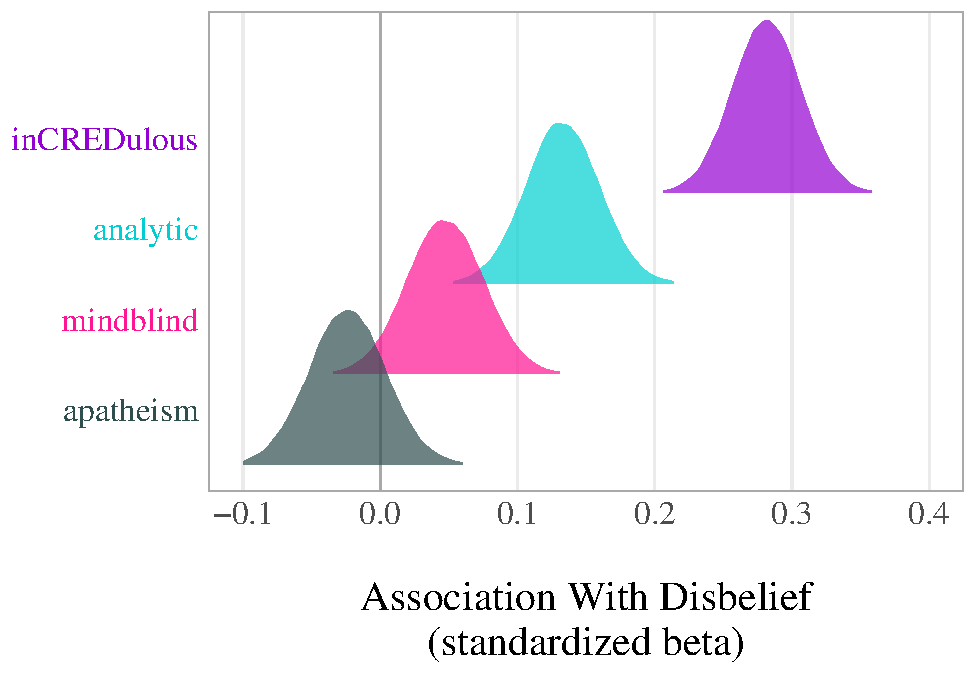
\includegraphics{papaja-version_files/figure-latex/posterior plot-1.pdf}
\caption{(\#fig:posterior plot)Posterior densities illustrating how strongly each factor predicts disbelief. Height in each density indexes credibility of estimate: values higher up each curve are better guesses.}
\end{figure}

\begin{table}[!h]

\caption{(\#tab:full model table)Predicting Disbelief: Full Model Summary}
\centering
\begin{tabular}[t]{lrrr}
\toprule
Variable & Beta & HPDI & Pr\\
\midrule
mindblind & 0.05 & [-0.01, 0.11] & 0.96\\
apatheism & -0.02 & [-0.08, 0.04] & 0.2\\
inCREDulous & 0.28 & [0.23, 0.34] & > 0.99\\
analytic & 0.13 & [0.07, 0.19] & > 0.99\\
\hspace{1em}Age & 0.01 & [-0.04, 0.07] & 0.67\\
\addlinespace
\hspace{1em}Education & 0.04 & [-0.02, 0.1] & 0.92\\
\hspace{1em}Male & 0.07 & [0.02, 0.13] & > 0.99\\
\hspace{1em}Social Lib & 0.44 & [0.35, 0.52] & > 0.99\\
\hspace{1em}Economic Cons & 0.04 & [-0.04, 0.12] & 0.84\\
\hspace{1em}Extraversion & 0.02 & [-0.03, 0.08] & 0.82\\
\addlinespace
\hspace{1em}Conscientiousness & 0.02 & [-0.04, 0.07] & 0.72\\
\hspace{1em}Neuroticism & 0.00 & [-0.06, 0.07] & 0.54\\
\hspace{1em}Low Agreeableness & 0.10 & [0.04, 0.17] & > 0.99\\
\hspace{1em}Openness & 0.07 & [0.02, 0.13] & > 0.99\\
\hspace{1em}Honesty/Humility & 0.04 & [-0.02, 0.1] & 0.92\\
\bottomrule
\multicolumn{4}{l}{\textit{Note: }}\\
\multicolumn{4}{l}{ }\\
\multicolumn{4}{l}{\textsuperscript{1} Beta = standardized beta}\\
\multicolumn{4}{l}{\textsuperscript{2} HPDI = 97\% Highest posterior density interval}\\
\multicolumn{4}{l}{\textsuperscript{3} Pr = posterior probability of Beta > 0}\\
\end{tabular}
\end{table}

\hypertarget{atheism-binary-measure}{%
\subsubsection{Atheism: Binary Measure}\label{atheism-binary-measure}}

We also measured religious disbelief with a simple binary (No, Yes) belief in God item. We reran our full model analysis as a logistic model predicting atheism rates on the binary measure. Results closely matched the continuous full model. Aside from demographic covariates, only fewer religious CREDs, \emph{beta} = 0.83, {[}0.61, 1.05{]}, \(\mathrm{P}(beta > 0 \mid data)\) = 1, and more cognitive reflection, \emph{beta} = 0.38, {[}0.17, 0.59{]} = \(\mathrm{P}(beta > 0 \mid data)\) = 1, predicted atheism. However, inCREDulous atheism was again much stronger than analytic atheism. To illustrate, we considered the posterior produced by our model, marginalized at various levels of our predictors. Specifically, we compared the hypothetical probability of atheism for model-predicted golems who are either perfectly inCREDulous (scoring at floor for religious CREDs) but typical on all other variables, or else perfectly analytical (scoring at ceiling on cognitive reflection) but otherwise typical. The predicted odds of atheism are about 90\% higher for the purely inCREDulous golem, \(\mathrm{P}(atheism \mid inCREDulous)\) = 0.31, {[}0.24, 0.39{]}, than for the purely analytic golem, \(\mathrm{P}(atheism \mid analytic)\) = 0.2, {[}0.13, 0.28{]}, \emph{odds ratio} = 1.87, {[}0.93, 3.03{]}, \(\mathrm{P}(inCREDulous > analytic \mid data)\) = 0.99. This relative difference in predictive strength for inCREDulous atheism and analytic atheism, replicated across continuous and binary measures of disbelief, is consistent with a dual inheritance approach.

\hypertarget{ii.-hypothesized-interactions}{%
\subsection{II. Hypothesized Interactions}\label{ii.-hypothesized-interactions}}

Next, we probed for preregistered interactions among the four factors\footnote{Preregistered analyses probing for interactions with mentalizing yielded nothing of particular note and are summarized in the Online Supplement.} finding an interaction between cultural learning and reflective cognitive style, \(\beta\) = -0.08, {[}-0.12, -0.03{]}, \(\mathrm{P}(\beta > 0 \mid data)\) = 1. We considered the association between disbelief and reflective cognitive style among those comparatively high and low on credible cultural cues of religious belief (Figure 2), finding that reflective cognitive style primarily predicts religious disbelief among those who were also comparatively low in cultural exposure to credible religious cues of faith. Indeed, cognitive reflection moderately predicted religious disbelief among those witnessing the fewest religious CREDs, \(\beta\) = 0.26, {[}0.15, 0.35{]}, \(\mathrm{P}(\beta > 0 \mid data)\) = 0, but not at all among those highest in religious CREDs, \(\beta\) = -0.01, {[}-0.13, 0.1{]}, \(\mathrm{P}(\beta > 0 \mid data)\) = 0.60. These patterns highlight the interactive predictive roles of cultural context and evolved intuitions on religious cognition, consistent with a dual inheritance perspective.

\begin{figure}
\centering
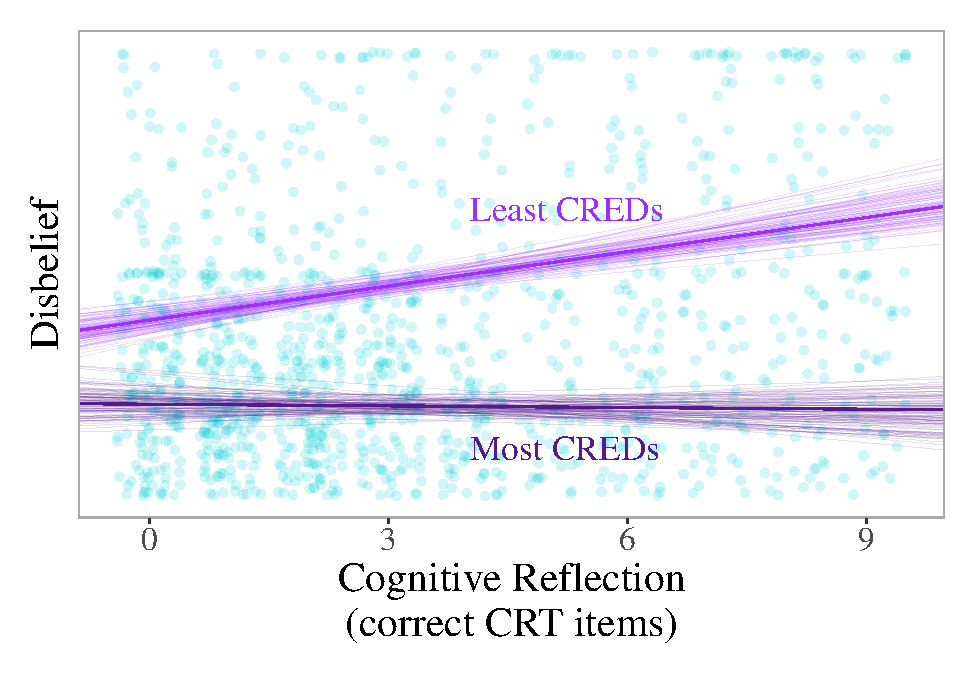
\includegraphics{papaja-version_files/figure-latex/interaction plot-1.pdf}
\caption{(\#fig:interaction plot)Cognitive reflection primarily predicts disbelief among individuals who are also relative low in exposure to religious CREDs. Each cluster contains 100 regression lines drawn from the posterior to illustrate estimate uncertainty and regions of highest posterior density. Y-axis depicts the entire range of possible values for the arbitrarily scaled continuous measure.}
\end{figure}

\hypertarget{iii.-individual-replications}{%
\subsection{III. Individual Replications}\label{iii.-individual-replications}}

Finally, we tested each candidate factor in isolation, merely to replicate in a nationally representative sample previous work that has independently correlated indices of mentalizing, existential security, religious CREDs, and cognitive style with various measures of religious belief. In individual zero-order replication analyses (Table 3), inCREDulous atheism, analytic atheism, and mindblind atheism largely replicated previous work. Apatheism was again not evident in this sample. That one of the candidate factors culled from existing literature did not appear as a robust predictor may suggest tempered enthusiasm for its utility as a predictor of individual differences in religiosity more broadly, although existential security is still quite useful in analyzing larger-scale regional and international trends ({\textbf{???}}).

\begin{table}[!h]

\caption{(\#tab:individual tables)Predicting Disbelief: Individual Replication Analyses}
\centering
\begin{tabular}[t]{lrrr}
\toprule
Variable & r & HPDI & Pr\\
\midrule
mindblind & 0.06 & [0, 0.12] & 0.99\\
apatheism & -0.03 & [-0.09, 0.02] & 0.1\\
inCREDulous & 0.38 & [0.32, 0.43] & >0.99\\
analytic & 0.18 & [0.13, 0.24] & >0.99\\
\bottomrule
\multicolumn{4}{l}{\textit{Note: }}\\
\multicolumn{4}{l}{ }\\
\multicolumn{4}{l}{\textsuperscript{1} HPDI = 97\% Highest posterior density interval}\\
\multicolumn{4}{l}{\textsuperscript{2} Pr = posterior probability of Beta > 0}\\
\end{tabular}
\end{table}

\hypertarget{discussion}{%
\section{Discussion}\label{discussion}}

\hypertarget{summary}{%
\subsection{Summary}\label{summary}}

Overall, we present one of the most comprehensive available analyses of the cognitive, cultural, and motivational factors that predict individual differences in religious belief and disbelief in the USA. These results speak directly to competing theoretical perspectives on the origins of religious disbelief culled from sociology, social psychology, evolutionary psychology, cognitive science of religion, cultural evolution, and gene-culture coevolution. Consistent patterns emerged, suggesting that the most potent predictor of disbelief is---by a wide margin---lack of exposure to credibility enhancing displays of religious faith. Once this context-biased cultural learning mechanism is accounted for, reflective cognitive style predicts some people being slightly more prone to religious disbelief than their cultural upbringing might otherwise suggest. That said, this relationship was relatively modest. Advanced mentalizing was a robust but weak predictor of religious belief, and existential security did not meaningfully predict disbelief. In terms of different disbelief pathways, inCREDulous atheism appears relatively strong and robust, analytic atheism is robust but modest, and there is robust evidence for a very small role of mindblind atheism.

\hypertarget{theoretical-implications}{%
\subsection{Theoretical Implications}\label{theoretical-implications}}

We evaluated predictions about the origins of disbelief from three prominent theoretical perspectives: secularization, cognitive byproduct, and dual inheritance. Comparing the predictions in Table 1 with the results of Figure 1, it is clear that our results are most consistent with the dual inheritance perspective. Indeed, this was the only theoretical perspective that predicted prominent roles for both inCREDulous atheism and analytic atheism. Given the primacy of cultural learning in our data, any model that does not rely heavily on context-biased cultural learning is likely a poor fit for explaining the origins of religious disbelief. By extension, such models are necessarily incomplete or faulty evolutionary accounts of religion. Simply growing up in a home with relatively fewer credible displays of faith predicted disbelief, contra prior assertions from the cognitive science of religion that disbelief results from \enquote{special cultural conditions} and \enquote{a good degree of cultural scaffolding} ({\textbf{???}}). Instead, disbelief emerges quite naturally and easily in the mere relative absence of repeated and credible cues of others' belief.

Analytic atheism is perhaps the most discussed avenue to disbelief in the literature ({\textbf{???}}; {\textbf{???}}; {\textbf{???}}) and broader culture ({\textbf{???}}), but its popularity greatly overstates its actual influence. Although in this sample overall there was consistent evidence of analytic atheism, the overall trend was modest, the trend itself varied considerably across exposure to CREDs, and sufficient religious CREDs predictively buffered believers against the putatively corrosive influence of reflective cognition on faith. Despite claims that atheism generally requires cognitive effort or reflection ({\textbf{???}}; {\textbf{???}}), analytic atheism---as in other recent work ({\textbf{???}})---does not appear to be an especially general or powerful phenomenon.

It is initially puzzling that existential security proved impotent in our analyses, as it appears to be an important factor in explaining cross-cultural differences in religiosity ({\textbf{???}}; barberCountryReligiosityDeclines2013; {\textbf{???}}). Further, it has been used successful in experimental work ({\textbf{???}}; {\textbf{???}}), although these experimental insights may be less robust than initially assumed ({\textbf{???}}). It is possible that our analyses were at the wrong level of analysis to capture the influence of existential security, which may act as a precursor to other cultural forces. There may actually be a two-stage generational process whereby existential security demotivates religious behavior in one generation, leading the subsequent generation to atheism as they do not witness credibility enhancing displays of faith. This longitudinal societal prediction merits future investigation.

Finally, this work has implications beyond religion. Presumably, many beliefs arise from an interaction between core cognitive faculties, motivation, cultural exposure, and cognitive style. The general dual inheritance framework adopted here may prove fruitful for other sorts of beliefs elsewhere. Indeed, a thorough exploration of the degree to which different beliefs are predicted by cultural exposure relative to other cognitive factors may be useful for exploring content- versus context-biased cultural learning, and the contributions of transmitted and evoked culture. As this is a prominent point of contention between different schools of human evolutionary thought ({\textbf{???}}), such as evolutionary psychology and cultural evolution, further targeted investigation may be productive.

\hypertarget{metascientific-implications}{%
\subsection{Metascientific Implications}\label{metascientific-implications}}

This work suggests three broader meta-scientific points.

First, it illustrates a sort of \emph{replication-plus} approach to forensically evaluating the literature while simultaneously testing and advancing theory. We conducted preregistered replications of four distinct findings from four different literatures, attesting to their relative strength or weakness. This is of course intrinsically valuable. However, these four replications gain theoretical significance when combined, as we were able to directly evaluate the predictive suitability of prominent theoretical perspectives on the origins of disbelief. This would not have been possible in separate direct replications. Replication-plus approaches like ours may prove similarly useful in other domains. Although a Registered Replication Report format, in which multiple labs conduct a single replication of a unique operationalization, has taken central stage in the psychology meta-science world, alternative approaches and viewpoints on replication and methodology may be beneficial ({\textbf{???}}; {\textbf{???}}), including this replication-plus approach, proof-of-concept paradigmatic replication ({\textbf{???}}), and radically randomized meta-studies ({\textbf{???}}). As methodological introspection in psychology proceeds, we urge epistemic diversity in approaches ({\textbf{???}}).

Second, of the four candidate factors we tested, one (credibility enhancing displays) is derived from formal theoretical modeling in gene-culture coevolution, while the other three emerged from verbal argumentation. In terms of predicting large-scale real-world patterns, the formally modeled approach empirically outclassed the three \enquote{veories.}\footnote{\enquote{veories} are verbal theories, the intuitive verbal models that predominate much of the social sciences.} Verbal theorizing is an important step in the research process, but formal theorizing is an indispensable tool as well ({\textbf{???}}). Formal models are obviously wrong, yet they are useful mental prostheses simply because they are precisely and transparently wrong ({\textbf{???}}; {\textbf{???}}). In contrast, veories invite flexibility in interpretation and subsequent research design and analysis, hampering true empirical and theoretical progress ({\textbf{???}}). Further development in theory can circumvent methodological challenges to replicability ({\textbf{???}}; {\textbf{???}}), sharpen thinking beyond statistical desiderada ({\textbf{???}}), and spur scientific discovery ({\textbf{???}}).

Third, most psychology research nowadays emerges from convenience samples of undergraduates and Mechanical Turk workers. These samples are fine for some purposes, quite limited for others ({\textbf{???}}), and are known to depart from representativeness ({\textbf{???}}; {\textbf{???}}). While our nationally representative sampling allows us to generalize beyond samples we can access for free (in lab) or cheap (MTurk), even a large nationally representative sample barely scratches the surface of human diversity ({\textbf{???}}; {\textbf{???}}). As such, we encourage similar analyses across different cultures ({\textbf{???}}). Indeed, the possible existence of a historically contingent relationship between certain religious norms and the origins of WEIRD psychology ({\textbf{???}}) underscores the potential sensitivity of these and similar results to cultural context. Diversifying the samples that make up the empirical portfolio of evolutionary approaches to religion is especially necessary because cultural cues themselves emerged as the strongest predictor disbelief in this and related work ({\textbf{???}}; {\textbf{???}}; {\textbf{???}}; {\textbf{???}}). If this general pattern holds across societies, we predict that---beyond religion---veories developed by WEIRD researchers to explain the weird mental states of WEIRD participants can only aspire to ever more precisely answer a mere outlier of an outlier of our most important scientific questions about human nature.

\hypertarget{coda}{%
\subsection{Coda}\label{coda}}

The importance of transmitted culture and context-biased cultural learning as a predictor of belief and disbelief cannot be overstated. Combined, the data we collected suggest that if you are guessing whether or not individuals are believers or atheists, you are better off knowing how their parents behaved---Did they tithe? Pray regularly? Attend synagogue?---than how they themselves process information. Further, our interaction analyses suggest that sufficiently strong cultural exposure yields sustained religious commitment, even in the face of the putatively corrosive influence of cognitive reflection. Theoretically, these results fit well within a dual inheritance approach, as evolved cognitive capacities for cultural learning prove to be the most potent predictor of individual differences in the cross-culturally canalized expression of religious belief. Atheists are becoming increasingly common in the world, not because human psychology is fundamentally changing, but rather because evolved cognition remains fairly stable in the face of a rapidly changing cultural context that is itself the product of a coevolutionary process. Faith emerges in some cultural contexts, and atheism is the natural result in others.

\pagebreak

\hypertarget{acknowledgements}{%
\section{Acknowledgements}\label{acknowledgements}}

This research was supported by a grant to the first author from the John Templeton Foundation (48275). The content is solely the responsibility of the authors and does not necessarily represent the official views of its funders. The funders had no role in study design, data collection and analysis, decision to publish or preparation of the manuscript.

\hypertarget{author-contributions}{%
\section{Author Contributions}\label{author-contributions}}

A1 designed the study, with survey revision and implementation from A2 and A3. A2 contributed feedback and piloting throughout the life of this project. A1 performed the primary analyses and A4 performed descriptive analyses. A1 wrote the manuscript with A4. All authors approved the final manuscript.

\hypertarget{ethics}{%
\section{Ethics}\label{ethics}}

This project was approved by the Office of Research Integrity.

\hypertarget{data-code-and-materials}{%
\section{Data, code and materials}\label{data-code-and-materials}}

All data, code, and materials are available at \url{https://github.com/wgervais/disbelief-origins} and \url{https://osf.io/kfasv}.

\pagebreak

\hypertarget{references}{%
\section{References}\label{references}}

\newpage

\hypertarget{references-1}{%
\section{References}\label{references-1}}

\begin{Shaded}
\begin{Highlighting}[]
\KeywordTok{r_refs}\NormalTok{(}\DataTypeTok{file =} \StringTok{"BAMLabLib.bib"}\NormalTok{)}
\end{Highlighting}
\end{Shaded}

\begingroup
\setlength{\parindent}{-0.5in}
\setlength{\leftskip}{0.5in}

\hypertarget{refs}{}

\endgroup

\end{document}
